\documentclass{acm_proc_article-sp}
\begin{document}
\title{Sorting algorithms - comparison and analysis }
\subtitle{ CS21120 2013-2014 Assignment 2 }
\numberofauthors{1}
\author{
\alignauthor
Evdzhan Mustafa\\
       \affaddr{Student at University of Aberystwyth, Wales}
       \email{enm3@aber.ac.uk}
}
\maketitle
\begin{abstract}
This paper compares 6 comparison-based and one address-based, sorting algorithms, in order to determine each algorithm's behaviour given specific amount of input. Based on the time complexity, algorithms differ a lot, so they were divided into subgroups and compared with each other, within the subgroups. The first sub group was concluded to be very slow for large data sets, although it still can find uses. The second sub group scales really well on large data sets. The final conclusion is that combination of the two can achieve best result for a general case sorting needs. The address based kind of sort is also discussed, but was concluded to be very limited to its use.
\end{abstract}
\category{D.2.8}{Software Engineering}{Metrics}[complexity measures, performance measures]
\terms{Algorithms, Performance}
\keywords{Bubble Sort,Insertion Sort,Merge Sort,Shell Sort,Selection Sort,Radix Sort,Quick Sort}
\section{Introduction}
Each algorithm will be tested with up to 23 files\footnote{Some algorithms are so slow that is not practical to use all the files}. The files contain numbers, and are in unordered state. For the given file, each algorithm's completion time will be recorded, and then compared with the other algorithms, or variation of the same algorithm. Furthermore, an algorithm will be tested with an input file, that will be in ascending or descending sorted state. That is to determine the algorithms behaviour to variations in the file.
\section{The {\secit Experiment }}
A program written in JAVA was used to record the running times of the tested algorithms. All the algorithms were tested in the same environment, with no other programs running in the background. An algorithm was deployed several times, and the average running time was calculated. For an algorithm, the average running time was recorded and shown in a chart. The units used in the Y-axis are seconds. The X-axis shows the input amount. Files 1 through 23 contain 1 000 up to 10 000 000 elements.
\section{Average case $O(n^2)$ algorithms}
\begin{figure}[!htb]
\centering
\caption{Improved Bubble Sort.}
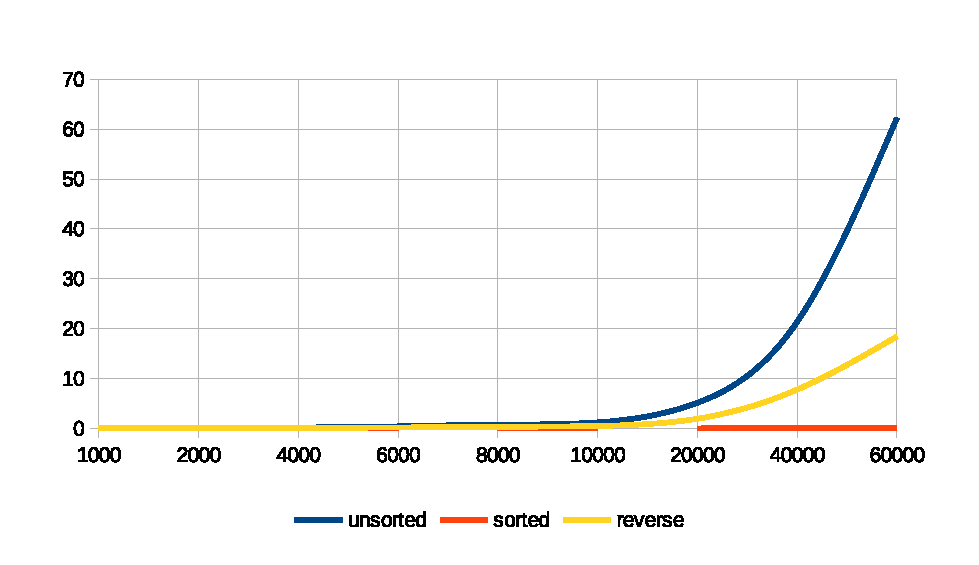
\epsfig{file=improved_bubble_sort.eps, height=2.5in, width=3.3in}
\end{figure}
\subsection{Bubble Sort}
A very bad sorting algorithm. Easy to implement, but terribly slow. Although it can be improved, the time complexity remains $O(n^2)$ . Due to the extremely big growth rate of Bubble sort, only the files containing up to 60 000 items are shown on the graph. It is impractical to run the tests for larger datasets. If an improved version is used on an already sorted array the time complexity drops down to  $O(n)$ - its best case. In such case, the algorithm essentially goes through every value once, without doing any swaps. An interesting fact is that if the data is reversed (i.e. sorted in descending order), the sorting is faster. This is because for every single comparison, a swap occurs. Whereas for random data, not all comparisons lead to a swap. This leads to more comparisons required to bring the data to a sorted state.
\subsection{Selection Sort}
It's average running time is similar to the one of the bubble sort, but is faster. It's con is that it is very easy to implement. The strategy used is to repeatedly go through the array and find the lowest value (select it).\\
 As seen on the graph, trying to sort already sorted array, takes less time. This is because no elements are moved. Only comparisons are performed to determine that the data is sorted. The majority of the time this algorithm runs in is to iterate over and over the array (to find the next lowest value). This is what causes it to be so slow for larger data sets. The reason Selection Sort is faster than Bubble Sort is that fewer swaps occur. This is because swap happens only when the next value is found, and is placed into it's correct and final position. Whereas in Bubble Sort, values are slowly "bubbled" to their correct position. \\\\\\
\begin{figure}[!htb]
\caption{Selection sort.}
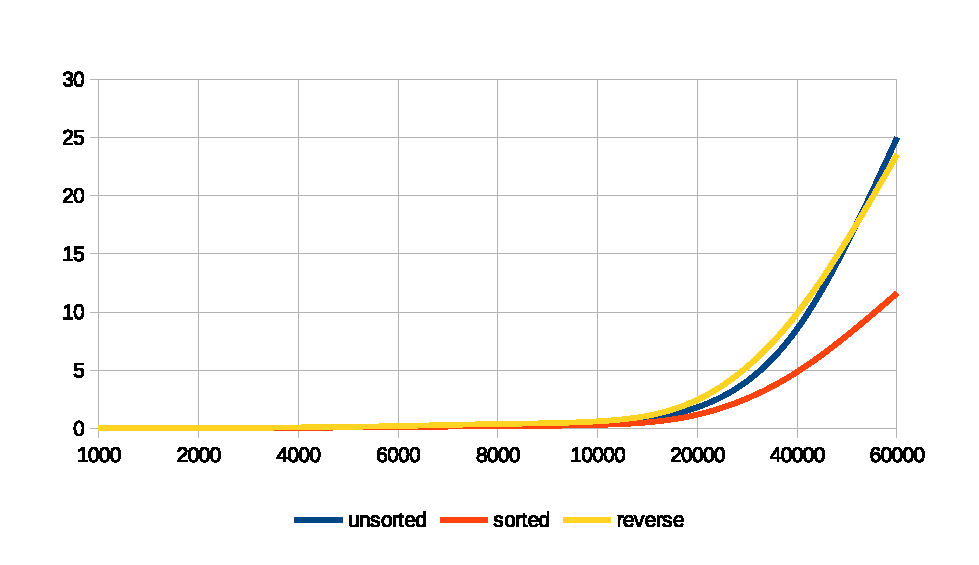
\epsfig{file=selection_sort.eps, height=2.5in, width=3.3in}
\end{figure}
\subsection{Insertion Sort}
\begin{figure}[h]
\caption{Insertion sort.}
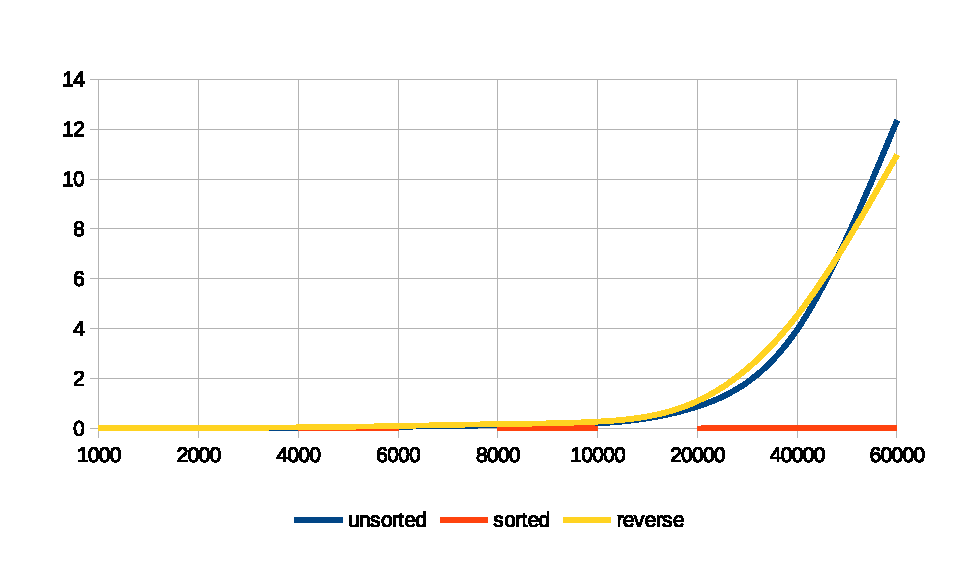
\epsfig{file=insertion_sort.eps, height=2.5in, width=3.3in}
\end{figure}
The insertion sort is the quickest of the three $O(n^2)$ algorithms. It's con is that it performs very quickly on small sets of data. As in the case with improved bubble sort, this algorithm can recognize if the initial array is already sorted. This leads to all loop iteration being skipped - that is its best case performance. Furthermore even if the array wasn't sorted completely, but rather nearly sorted, it would still cause many loop iterations to be skipped. This is why  insertion sort finds application in hybrid sorting algorithms.One of the drawbacks of this algorithm is that it repeatedly has to shift certain amount of elements to insert the current element to its correct place. This is the part where it spends most of its running time. The graph clearly shows that the time taken for a sorted array is negligible. That is not a single shift operation has happened, but only comparisons.
\subsection{$O(n^2)$ algorithms discussion} 
\begin{figure}[h]
\caption{Improved Bubble, Selection and Insertion sorts.}
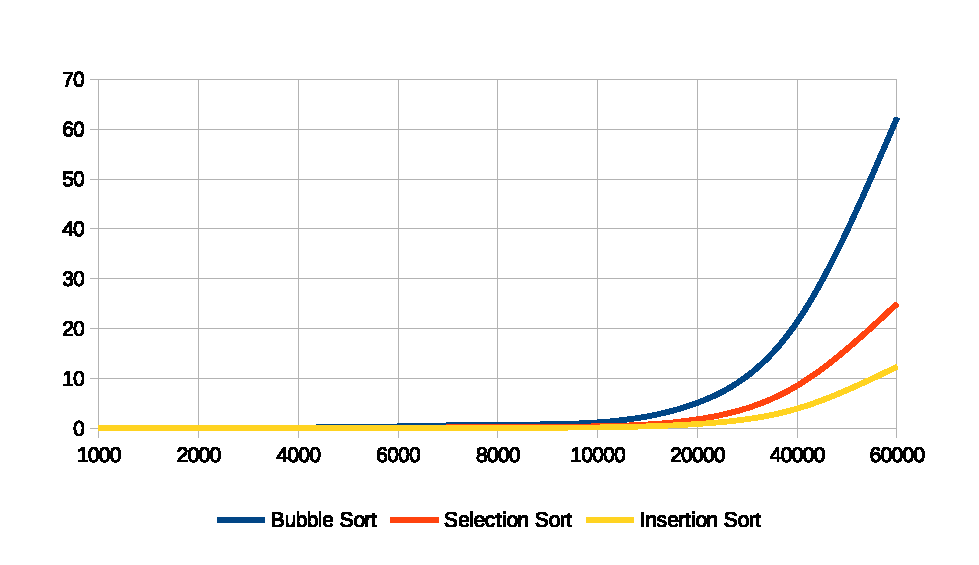
\epsfig{file=n2sorts.eps, height=2.5in, width=3.3in}
\end{figure}
Figure 4 shows  Bubble, Selection and Insertion sorts with their performance for unsorted data,for up to 60 000 elements. As seen on the figure, the performance time of the three $O(n^2)$ discussed so far, grows really quickly.  The time complexity is obviously not linear. The reason for this is that to find an element's correct and final place it takes N time. This is repeated for all N elements. \\ In the next doubling of the input amount, all of them take more than a minute to finish. This makes them impractical for large amounts of data. However they can still have some use. When the data to be sorted is less than 1000, the time taken is negligible. Furthermore, as mentioned earlier, they can be used in hybrid sorts, because they act much faster on already sorted, or nearly sorted data sets.
\section{Average case $O(n \log_2 n)$ algorithms} 
\subsection{Quick Sort}
One of the fastest sorting algorithms. Sorts the array by finding each element's correct position. The currently sorted element is called the pivot. It's final position is determined by moving all the elements less and greater than it in two sub arrays. Then the sub arrays, are recursively quick-sorted. On returning the pivot and the two sub arrays are merged together. Usually, the described approach above is not implemented by directly creating additional arrays, but rather indexing the original array appropriately.
I have omitted explaining how is the pivot chosen in first place. It is very important to decide what strategy is going to be used for the pivot choice. If the pivot is not chosen wisely, quick sort can become a $O(n^2)$ algorithm quite easily. Figure 5 shows the behaviour of quick sort, where the pivot is the middle element between the first and last elements. It can be seen that if the input data is sorted, or reverse sorted, quick sort is faster.\\
\begin{figure}[!htb]
\caption{Quick sort. Pivot middle element.}
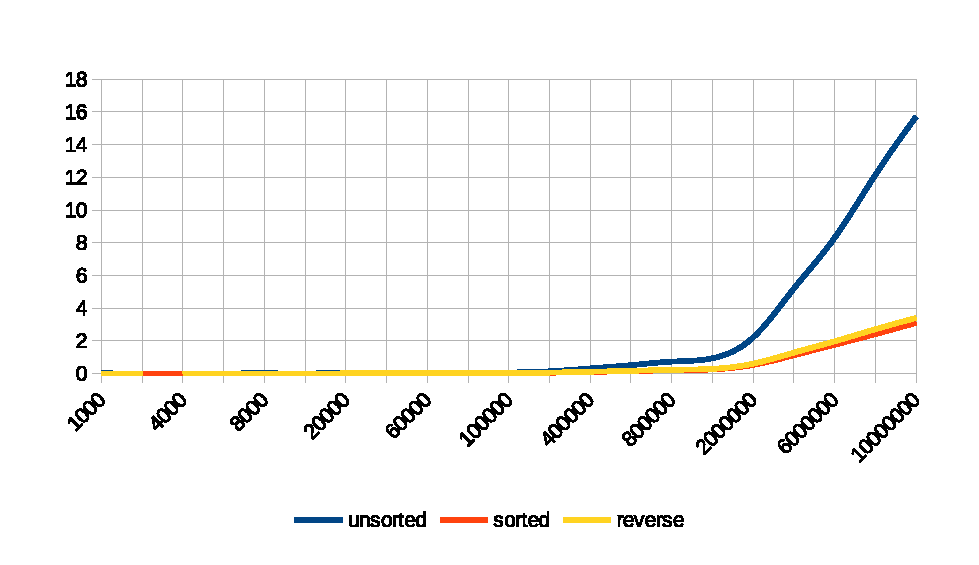
\epsfig{file=quick_sort_0.eps, height=2.5in, width=3.3in}
\end{figure}
\begin{figure}[!htb]
\caption{Quick sort. Pivot median.}
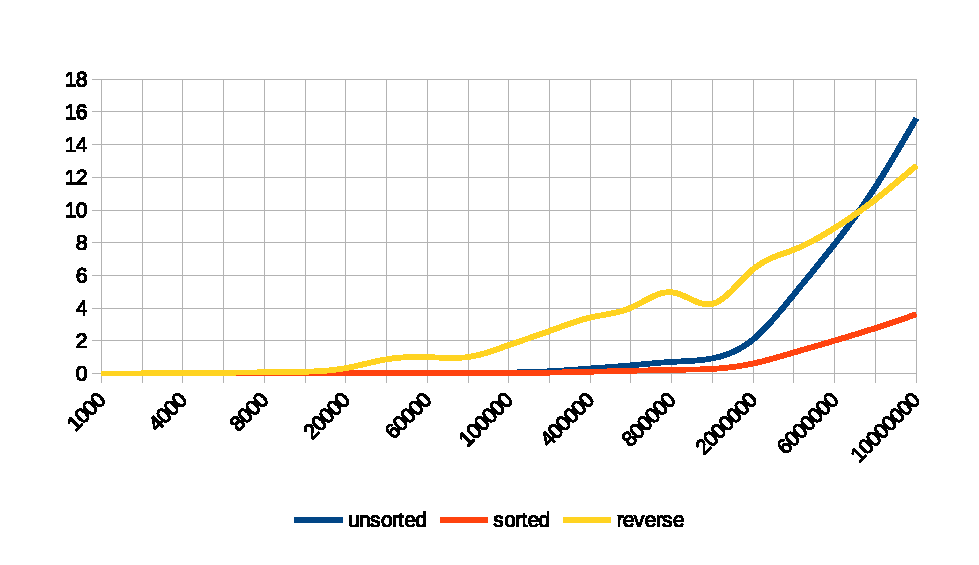
\epsfig{file=quick_sort_1.eps, height=2.5in, width=3.3in}
\end{figure}
\begin{figure}[!htb]
\caption{Quick sorts.}
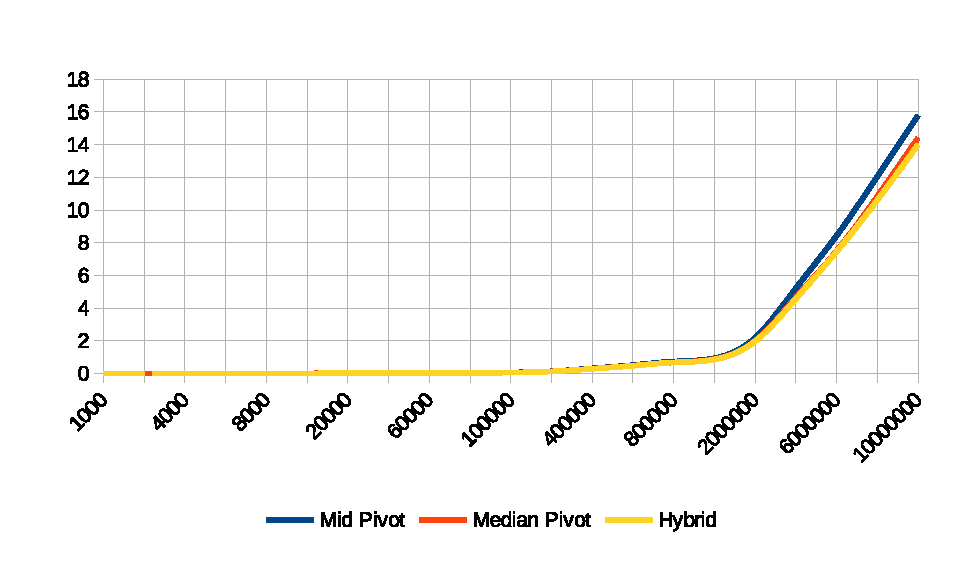
\epsfig{file=quick_sorts.eps, height=2.5in, width=3.3in}
\end{figure}
Now let's change the choice of the pivot. Let the pivot be the Median among the first, middle and last elements.
For unsorted data, the time taken to sort drops quite a bit - by about 2 seconds. However the reverse order performance increases drastically. For sorted data it doesn't make any difference.\\
There are various options for selecting the pivot. The best way to choose a pivot, depends on the data input. Some quick-sort versions are better for random data, some are better for almost sorted data.\\
Apart from the pivot choice, Quick Sort can be improved even more, by breaking the quick sort recursion when the smallest sub arrays to be sorted are of size 10 or less. In such case, the sorting can be finished off with Insertion Sort. In doing so, the overall algorithm performs slightly better. The time taken to sort drops by about 0,5 seconds for 10 million elements. Due to limitation of the machine used to run the tests, larger datasets could not be used. But those 0.5 seconds tells us that in next doubling of the data the difference will become bigger, thus the algorithm becomes more and more efficient as the data increases. Figure 7 shows comparison of the three Quick Sort flavours.

\subsection{Merge Sort}
\begin{figure}[!htb]
\caption{Merge Sort.}
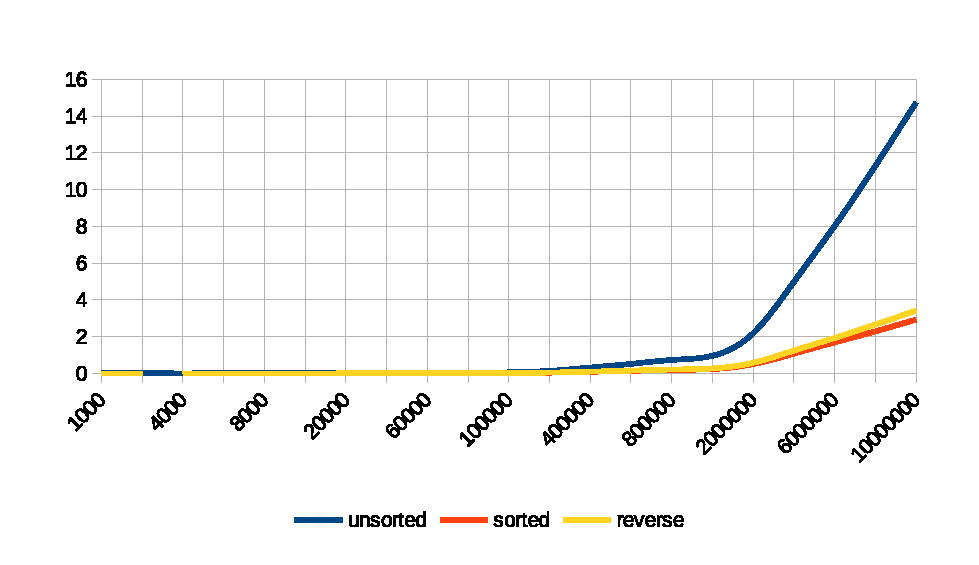
\epsfig{file=merge_sort.eps, height=2.5in, width=3.3in}
\end{figure}
Merge sort is another  $O(n \log_2 n)$ algorithm. It achieves similar result as quick sort, but has the overhead of requiring extra space. This is because the initial array that is to be sorted, is continually divided into halves, until arrays of 1 element are left. Then, each sub array value, is copied in the parent array taking the least values first. Yet again, this algorithm is recursive, and for smaller arrays it makes more sense to use simpler $O(n^2)$ algorithms such as Insertion sort. Figure 8 shows the performance of Merge sort - it is very similar to Quick Sort.\\

\subsection{Shell Sort}
Shell sort is a very clever $O(n \log_2 n)$ algorithm, because it does not require recursion. The sorting is done by introducing a variable N ($gap$). Elements that are N values apart, are compared, and swapped if necessary. After this iteration, the array is said to be N sorted. This guarantees that every Nth value is less than the next Nth value.
Then N is lowered by some criteria. And then another iteration occurs. This is done until the gap becomes 1, thus becoming a bubble sort, which is really quick on almost sorted data. 
\begin{figure}[!htb]
\caption{Shell Sort.}
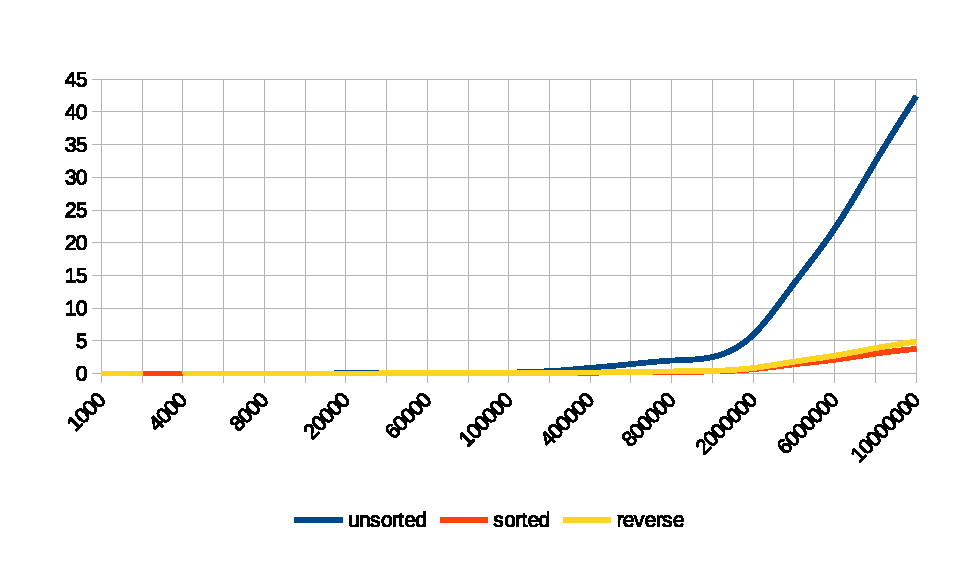
\epsfig{file=shell_sort.eps, height=2.5in, width=3.3in}
\end{figure}
Now what about the initial gap value ? And by what criteria is the gap lowered? As in Quick Sort's choice of pivot, how we choose the gaps are quite important. There various ways of choosing the set of gap values. And different sets, yield different results. However it is important that eventually the gap value drops to 1, so that the array is sorted correctly.  Figure 9 shows Shell Sort, with gap value initially equal to half the size of the array. Every next gap value is the previous divided by $2.2$ . This paper will not further elaborate on the choice of gap values and the changes, as it is quite deep topic.
\subsection{$O(n \log_2 n)$ algorithms discussion}
\begin{figure}[!htb]
\caption{$O(n \log_2 n)$ algorithms.}
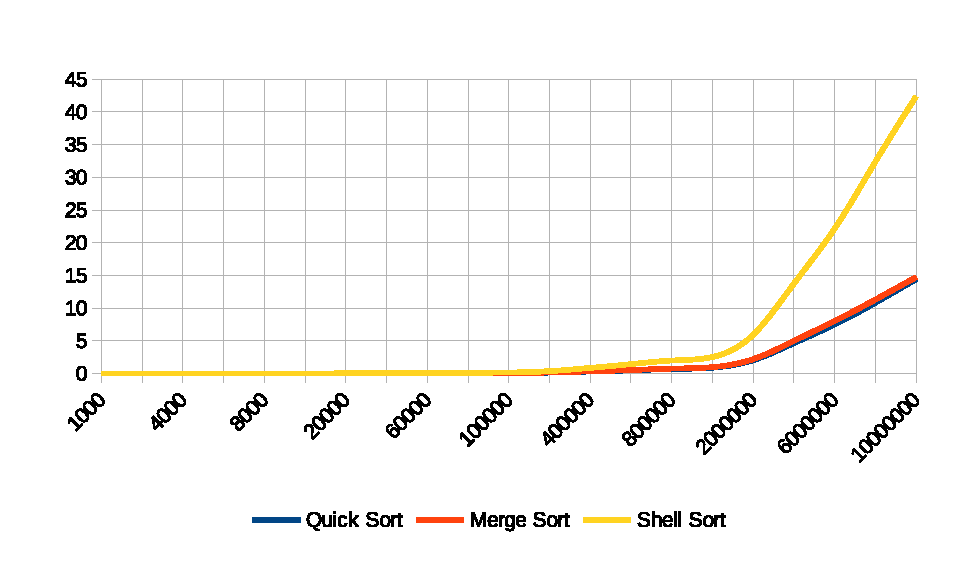
\epsfig{file=nlognsorts.eps, height=2.5in, width=3.3in}
\end{figure}
Figure 10 shows the comparison between previously discussed Quick Sort(median pivot), Merge Sort and Shell Sort for unsorted data. Merge and Quick sorts behave equally well. They do much better than Shell Sort. But that has a price - they both use recursion.  One thing to notice here is that Merge Sort requires linear extra space for the sorting. While Quick Sort doesn't require additional memory, it can become $O(n^2)$ complex if not implemented correctly. The time taken to find an element's correct and final position, for Quick Sort, and Merge Sort, is $log_2 N$. This is repeated for all N elements. For Shell Sort, the gap sequence is a major factor of how the algorithm will perform.\\\\\\\\
 
\section{Address based algorithms}
All the of the 6 algorithms covered so far were comparison-based. That is they compare two elements to determine which is greater. There is also another kind of sorting - address based. Let's examine Radix Sort - an address-based algorithm.\begin{figure}[!htb]
\caption{Radix sort.}
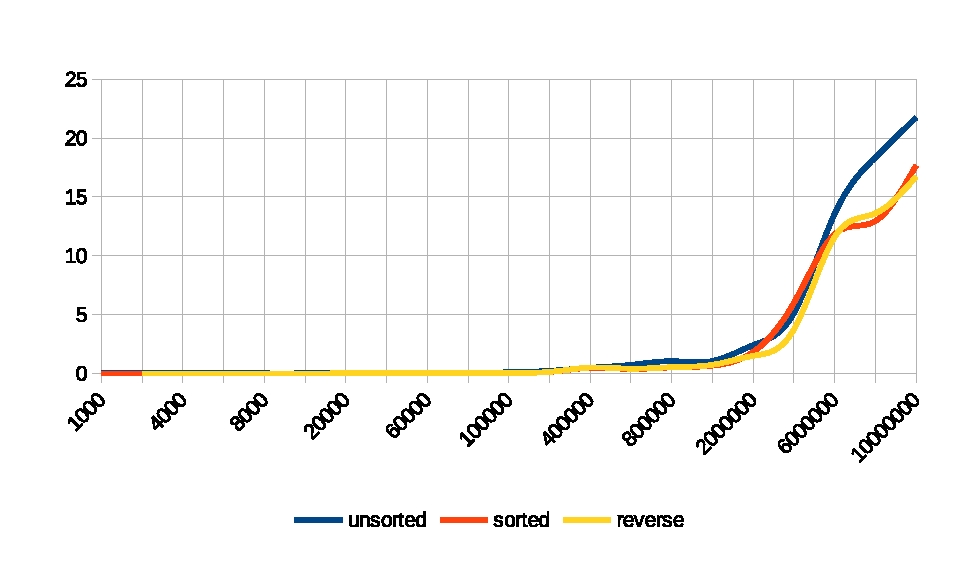
\epsfig{file=radix_sort.eps, height=2.5in, width=3.3in}
\end{figure}
Simply put, the array is sorted by putting arrays with same most significant digit in one place - an additional sub arrays. Then sort the sub array in the same manner, but using the next most significant digit. This uses tremendous amount of additional memory.  It is curious to notice how the slopes for reverse and sorted arrays, stay steady for some time periods,and then increase again. This is because more more bits are added to the greater values. It shows us that the time complexity is connected with the number of digits of the numbers sorted. Apart for numbers, address based algorithms have little use. They cannot be used on different type of objects. Although we used as an example numbers, any data set that has rules to determine which element is greater, can be sorted using comparison-based sorting. Whereas address-based is limited.\\
\section{Summary and Conclusion}
So far the best general purpose algorithm for big datasets is Quick Sort. Although it performs equally well as Merge Sort, it does not have the overhead of using additional memory. On the other hand, if our data is not that big, it is perfectly fine to use on of the slower sorts, such as Insertion. \\
We can combine the two ideas and produce an agile sorting algorithm that uses $O(n \log_2 n)$ sort when the data set is large, and switch to $O(n^2)$ sort, when the data is small. This idea was shown when Quick Sort was discussed, although the difference is not that big, it increases the efficiency more and more as the data grows. The clear winner is Quick Sort combined with Selection Sort - it is clever enough to sort with Insertion Sort, if the data is small, and scales really well for large data.

\bibliographystyle{abbrv}
\bibliography{sigproc} 
\appendix
\section{Acknowledgements}
Richard Shipman - provided the Radix and Bubble sort implementations.
\subsection{Materials used}
http://www.sorting-algorithms.com/ - Great website with pseudo-code describing algorithms. \\
http://en.wikipedia.org/wiki/Sorting\_algorithm  - Another website with theory and explanations about algorithms. \\
\section{Headings in Appendices}
\subsection{Introduction}
\subsection{The experiment}
\subsubsection{Best case $O(n^2)$ algorithms.}
\paragraph{Compare and discuss $O(n^2)$ sorting algorithms. }
\subsubsection{Best case $O(n \log_2 n)$ algorithms.}
\paragraph{Compare and discuss $O(n \log_2 n)$ sorting algorithms. }
\subsubsection{Address based algorithms}
\subsection{Summary and Conclusion}
\subsection{Acknowledgements}
\subsection{Materials used}
\end{document}
